\documentclass{article}

\usepackage{fancyhdr}
\usepackage{extramarks}
\usepackage{amsmath}
\usepackage{amsthm}
\usepackage{amsfonts}
\usepackage{tikz}
\usepackage[plain]{algorithm}
\usepackage{algpseudocode}
\usepackage{enumerate}
\usepackage{graphicx}
\usepackage{pythonhighlight}
\usepackage{amssymb}

\usetikzlibrary{automata,positioning}

%
% Basic Document Settings
%  

\topmargin=-0.45in
\evensidemargin=0in
\oddsidemargin=0in
\textwidth=6.5in
\textheight=9.0in
\headsep=0.25in

\linespread{1.1}

\pagestyle{fancy}
\lhead{\hmwkAuthorName}
\chead{\hmwkClass\ (\hmwkClassInstructor): \hmwkTitle}
\rhead{\firstxmark}
\lfoot{\lastxmark}
\cfoot{\thepage}

\renewcommand\headrulewidth{0.4pt}
\renewcommand\footrulewidth{0.4pt}

\setlength\parindent{0pt}

%
% Create Problem Sections
%

\newcommand{\enterProblemHeader}[1]{
    \nobreak\extramarks{}{Problem \arabic{#1} continued on next page\ldots}\nobreak{}
    \nobreak\extramarks{Problem \arabic{#1} (continued)}{Problem \arabic{#1} continued on next page\ldots}\nobreak{}
}

\newcommand{\exitProblemHeader}[1]{
    \nobreak\extramarks{Problem \arabic{#1} (continued)}{Problem \arabic{#1} continued on next page\ldots}\nobreak{}
    \stepcounter{#1}
    \nobreak\extramarks{Problem \arabic{#1}}{}\nobreak{}
}

\setcounter{secnumdepth}{0}
\newcounter{partCounter}
\newcounter{homeworkProblemCounter}
\setcounter{homeworkProblemCounter}{1}
\nobreak\extramarks{Problem \arabic{homeworkProblemCounter}}{}\nobreak{}

%
% Homework Problem Environment
%
% This environment takes an optional argument. When given, it will adjust the
% problem counter. This is useful for when the problems given for your
% assignment aren't sequential. See the last 3 problems of this template for an
% example.
%
\newenvironment{homeworkProblem}[1][-1]{
    \ifnum#1>0
        \setcounter{homeworkProblemCounter}{#1}
    \fi
    \section{Problem \arabic{homeworkProblemCounter}}
    \setcounter{partCounter}{1}
    \enterProblemHeader{homeworkProblemCounter}
}{
    \exitProblemHeader{homeworkProblemCounter}
}

%
% Homework Details
%   - Title
%   - Due date
%   - Class
%   - Section/Time
%   - Instructor
%   - Author
%

\newcommand{\hmwkTitle}{Homework\ \#1}
\newcommand{\hmwkDueDate}{November 22, 2020}
\newcommand{\hmwkClass}{Computational science and engineering}
\newcommand{\hmwkClassInstructor}{Professor Qifeng Liao}
\newcommand{\hmwkAuthorName}{Tianyuan Wu}
\newcommand{\hmwkAuthorID}{63305667}

%
% Title Page
%

\title{
    \vspace{2in}
    \textmd{\textbf{\hmwkClass:\ \hmwkTitle}}\\
    \normalsize\vspace{0.1in}\small{Due\ on\ \hmwkDueDate\ at 11:59pm}\\
    \vspace{0.1in}\large{\textit{\hmwkClassInstructor}}
    \vspace{3in}
}

\author{\textbf{\hmwkAuthorName}\\ \hmwkAuthorID}
\date{}

\renewcommand{\part}[1]{\textbf{\large Part \Alph{partCounter}}\stepcounter{partCounter}\\}

%
% Various Helper Commands
%

% Useful for algorithms
\newcommand{\alg}[1]{\textsc{\bfseries \footnotesize #1}}

% For derivatives
\newcommand{\deriv}[1]{\frac{\mathrm{d}}{\mathrm{d}x} (#1)}

% For partial derivatives
\newcommand{\pderiv}[2]{\frac{\partial}{\partial #1} (#2)}

% Integral dx
\newcommand{\dx}{\mathrm{d}x}

% Alias for the Solution section header
\newcommand{\solution}{\textbf{\large Solution}}

% Probability commands: Expectation, Variance, Covariance, Bias
\newcommand{\E}{\mathrm{E}}
\newcommand{\Var}{\mathrm{Var}}
\newcommand{\Cov}{\mathrm{Cov}}
\newcommand{\Bias}{\mathrm{Bias}}

\begin{document}

\maketitle

\pagebreak

\begin{homeworkProblem}
    Show the Gibbs phenomenon\\
    \solution\\
    In this problem, I use \texttt{python} to show the 
    fourier series of $step(x)$ in range $[0, 1]$. 
    We know that 
    $$s(x) = \sum_{k=1}^{\infty}{\frac{2}{\pi}\cdot h_k\cdot sin(kx)}$$
    where 
    $$h_k = \begin{cases}
        0, \quad \text{k is even}\\
        \frac{2}{k}, \quad \text{k is odd}
    \end{cases}$$
    and for delta function ($\delta(x)$):
    $$\delta(x) = \sum_{k=1}^{\infty}{\frac{1}{\pi}\cdot sin(kx)}$$
    The following diagram shows the fourier sums when $k=1$, $k=10$, $k=100$ and $k=500$ of step function and delta function.
    We can observe that when $x=0$ and $x=\pi$, the Fourier series has large oscillations near the jump
    (Gibbs phenomenon).
    \begin{figure}[H]
        \centering
        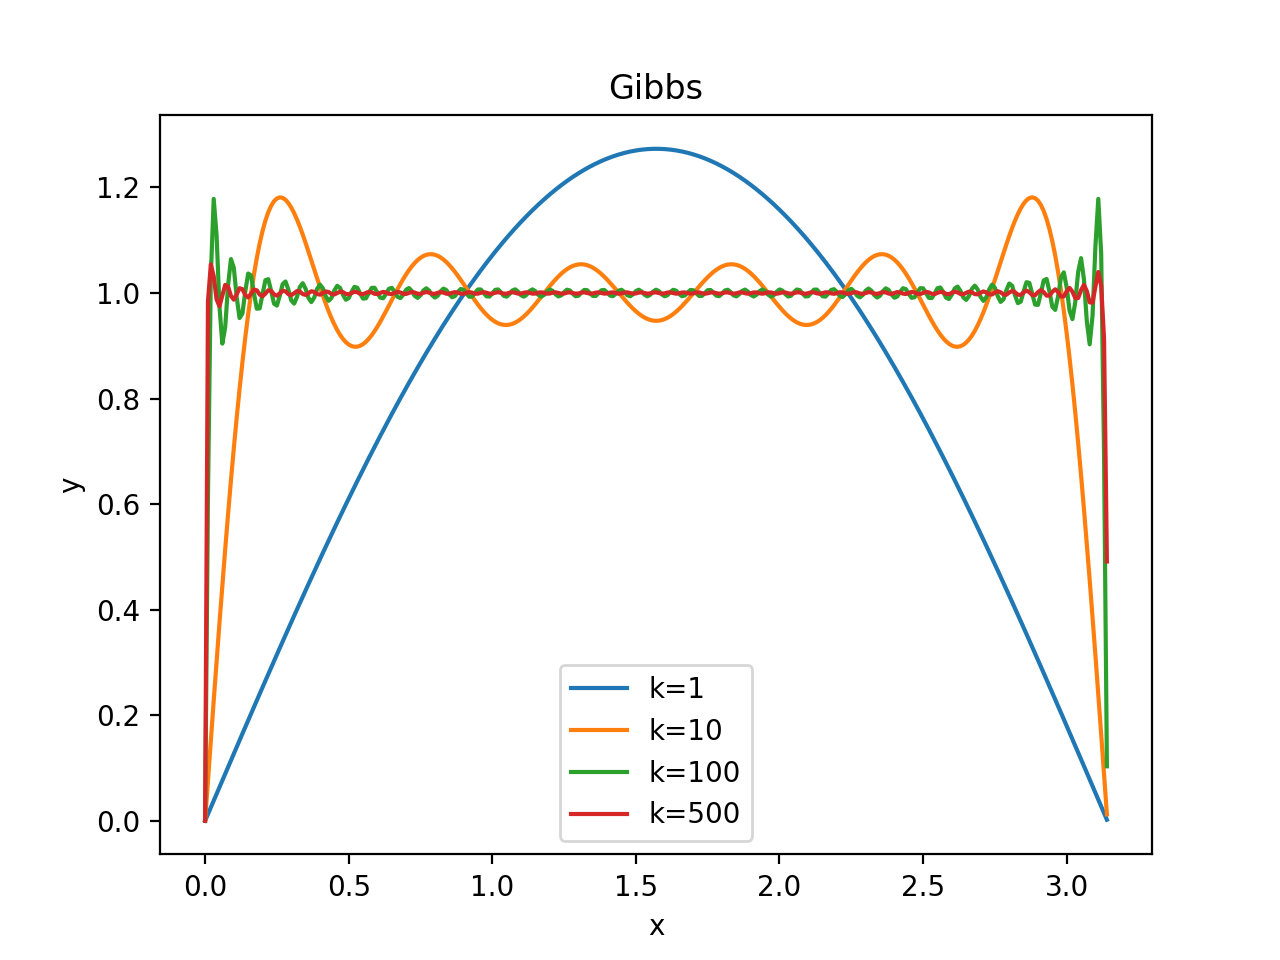
\includegraphics[scale=0.8]{gibbs.png}
        \caption{Gibbs phenomenon - step function}
    \end{figure}
    \begin{figure}[H]
        \centering
        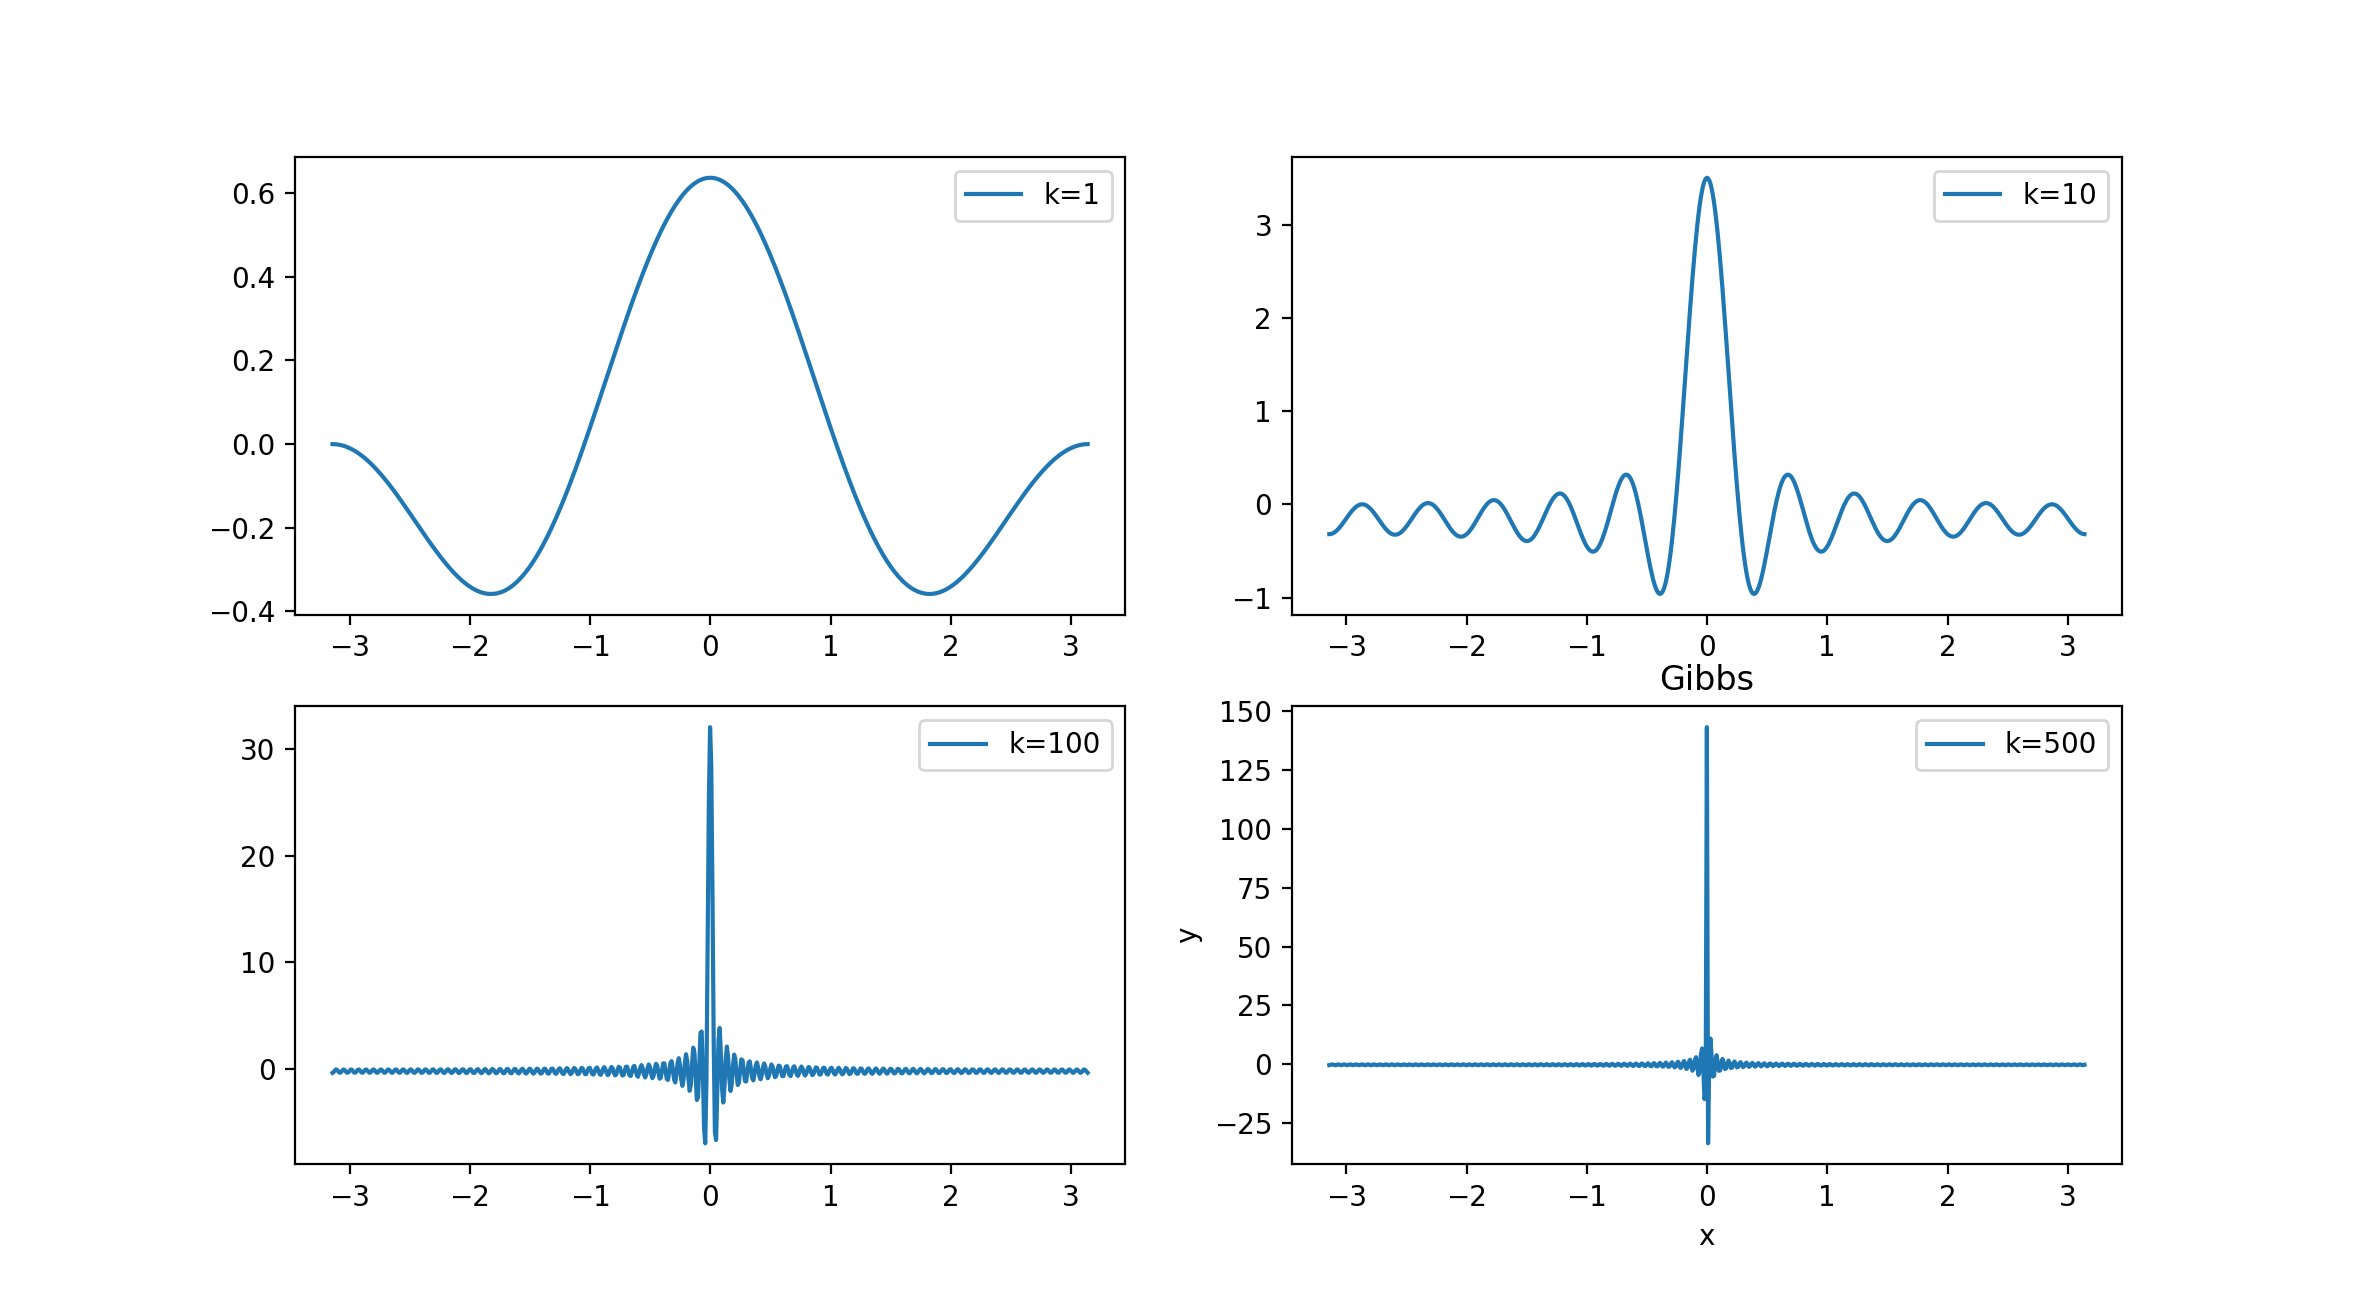
\includegraphics[scale=0.5]{delta.png}
        \caption{Gibbs phenomenon - delta function}
    \end{figure}
\end{homeworkProblem}

\newpage

\begin{homeworkProblem}
    Problem 4.1 on textbook\\
    \solution\\
    \begin{enumerate}
        \item[(a)] $f(x) = sin^3(x)$\\
            $$a_k = \frac{2}{\pi}\int_{-\pi}^{\pi}{}dx $$
        \item[(b)] $f(x) = |sin(x)|$\\
        
        \item[(c)] $f(x) = x$\\
        
        \item[(d)] $f(x) = e^x$, complex form\\
            $$a_k = sinh(x)$$
    \end{enumerate}
\end{homeworkProblem}

\end{document}
